\chapter{Arhitektura i dizajn sustava}

		{Prilikom projektiranja samog sustava jedna od važnijih odluka bila je odabir programskih jezika i razvojnih okruženja u kojima ćemo razviti našu aplikaciju. Programski jezici koje smo odabrali su Java sa Spring Boot razvojnim okvirom za \textit{backend} te React Javascript za \textit{frontend}. Odabrana razvojna okruženja su Eclipse za \textit{backend} te Visual Studio Code za \textit{frontend}.}	\\
		
		{Također izbor odgovarajuće arhitekture programske potpore jedan je od najbitnijih koraka u oblikovanju sustava jer ona predstavlja poveznicu između zahtjeva u sustav i same implementacije sustava. Dobra arhitektura znači dobru fleksibilnost sustava, jednostavnu mogućnost nadogradnje i jeftino održavanje.}\\
		
		{Sama arhitektura sustava je vrlo jednostavna, a sastoji se od dvije manje aplikacije: klijenta i poslužitelja. Osnovna prednost modela klijent-poslužitelj je u tome što nije potreban sustav za upravljanje bazom podataka na svakom klijentskom računalu, već se klijent s bazom podataka povezuje preko aplikacije. Time se postiže veća sigurnost i zaštita podataka. Poslužiteljska aplikacija ima pristup bazi podataka u kojoj će se pohranjivati podaci o lokacijama, kartama, borbama, igračima i kartografima. Poslužiteljska aplikacija neće dohvaćati slike i pohranjivati ih u bazu podataka već na servis Cloudinary. Poslužiteljska aplikacija temeljena je na REST principima za izradu web aplikacija te u skladu s time klijentska aplikacija dohvaća podatke iz poslužiteljske i prezentira ih na korisniku razumljiv način.}\\
		
		{Za izradu aplikacije odabrali smo MVC arhitekturu jer omogućava dodatno strukturiranje aplikacije s obzirom na objektno orijentiranu paradigmu što znatno olakšava nezavisni razvoj, ispitivanje i održavanje aplikacije.}		

				
		\section{Baza podataka}
			
			Podatci potrebni za funkcioniranje naše aplikacije pohranjuju se u relacijsku bazu podataka. Osnovni objekt relacijske baze podataka je relacija - imenovana dvodimenzionalna tablica čiji stupci predstavljaju atribute, a retci opisuju entitete baze podataka (retci u relaciji zovu se n-torke).
			Sljedeći entiteti sačinjavaju bazu podataka naše aplikacije:
			\begin{packed_item}
				\item Igrač (\textit{player})
				\item Zabrana pristupa (\textit{ban})
				\item Potvrda registracije (\textit{confirmation})
				\item Kartograf (\textit{mapper})
				\item Administrator (\textit{admin})
				\item Borba (\textit{fight})
				\item Lokacija (\textit{location})
				\item Najkraći put (\textit{path})
				\item Kategorija lokacije (\textit{category})
				\item Karta (\textit{card})
			\end{packed_item}
			
			\subsection{Opis tablica}
			
				\noindent\textbf{player} $($Igrač$)$ - Ovaj entitet sadržava podatke o korisniku. Svaki korisnik je ujedno i igrač. Sadrži atribute: ID korisnika, korisničko ime, hash lozinke, e-mail adresu, fotografiju, bodove igrača, status bana, aktivnost igrača, osposobljenost računa i "experience points". Ovaj entitet je u \textit{One-to-Many} vezi s entitetom card preko atributa player\_id. Ima dvije \textit{One-to-Many} veze s entitetom fight, koje se odnose na borbe u kojima je igrač pobijedio i borbe u kojima je izgubio. Player je u \textit{One-to-One} vezi s entitetom ban i s entitetom confirmation. \\
				
				Atribut username je alternativni ključ entiteta. Atribut ban\_status može poprimiti jednu od sljedećih vrijednosti: 0 - korisnik nije pod banom (nije isključen iz igre$)$, 1 - korisnik je privremeno isključen iz igre, 2 - korisnik je trajno isključen iz igre.
				
				\begin{longtabu} to \textwidth {|X[6, l]|X[7, l]|X[20, l]|}
					
					\hline \multicolumn{3}{|c|}{\textbf{player}}	 \\[3pt] \hline
					\endfirsthead
					
					\hline \multicolumn{3}{|c|}{\textbf{player}}	 \\[3pt] \hline
					\endhead
					
					\hline 
					\endlastfoot
					
					\cellcolor{LightGreen}\textbf{player\_id} & UUID 	&  	jedinstveni brojčani identifikator korisnika 	\\ \hline
					username & VARCHAR(32) 	&  	jedinstveno korisničko ime 	\\ \hline
					pass\_hash & VARCHAR(64)  &   hash lozinke \\ \hline 
					email & VARCHAR(128)  &   jedinstvena e-mail adresa korisnika \\ \hline 
					photo\_link & VARCHAR(200) & fotografija (avatar$)$ korisnika \\ \hline 
					points & INT	&  	broj bodova igrača	\\ \hline
					ban\_status & INT	&  	status o zabranama igrača	\\ \hline 
					activity & BOOLEAN	&  	oznaka je li igrač online	\\ \hline 
					enabled & BOOLEAN	&  	oznaka je li igraču omogućeno korištenje računa nakon registracije	\\ \hline
					experience	& INT	&	 mjera "iskustva" u igri iskazana brojčanom vrijednošću \\ \hline
					
				\end{longtabu}
			
				\noindent\textbf{confirmation} $($Potvrda registracije$)$ - Ovaj entitet sadržava podatke o potvrdi registracije. Sadrži atribute: ID tokena, token i ID korisnika. Ovaj entitet u vezi je \textit{One-to-One} s Player preko jedinstvenog brojčanog identifikatora korisnika.
				
				\begin{longtabu} to \textwidth {|X[6, l]|X[7, l]|X[20, l]|}
					
					\hline \multicolumn{3}{|c|}{\textbf{confirmation}}	 \\[3pt] \hline
					\endfirsthead
					
					\hline \multicolumn{3}{|c|}{\textbf{confirmation}}	 \\[3pt] \hline
					\endhead
					
					\hline 
					\endlastfoot
					
					\cellcolor{LightGreen}\textbf{token\_id} & UUID 	&   jedinstveni brojčani identifikator registracije 	\\ \hline
					token & VARCHAR(255) & token potvrde o registraciji\\ \hline
					\cellcolor{LightBlue}\textit{player\_id} & UUID 	&   jedinstveni brojčani identifikator korisnika 	\\ \hline  
					
				\end{longtabu}
			
				\noindent\textbf{ban} $($Zabrana pristupa$)$ - Ovaj entitet sadržava podatke o igračima kojima je zabranjen pristup aplikaciji. Sadrži atribute kraj zabrane i ID igrača. Ovaj entitet u vezi je \textit{One-to-One} s korisnikom (player$)$ preko ID-a korisnika.
				
				\begin{longtabu} to \textwidth {|X[6, l]|X[6, l]|X[20, l]|}
					
					\hline \multicolumn{3}{|c|}{\textbf{ban}}	 \\[3pt] \hline
					\endfirsthead
					
					\hline \multicolumn{3}{|c|}{\textbf{ban}}	 \\[3pt] \hline
					\endhead
					
					\hline 
					\endlastfoot
					
					\cellcolor{LightBlue}\textit{player\_id} & UUID 	&   jedinstveni brojčani identifikator igrača 	\\ \hline 
					ban\_end & DATE & datum isteka zabrane \\ \hline 
					
				\end{longtabu}
				
				\noindent\textbf{mapper} $($Kartograf$)$ - Entitet mapper nasljeđuje entitet player. Ovaj entitet, uz atribute playera, ima i atribute IBAN i ID photo.
				
				\begin{longtabu} to \textwidth {|X[6, l]|X[7, l]|X[20, l]|}
					
					\hline \multicolumn{3}{|c|}{\textbf{mapper}}	 \\[3pt] \hline
					\endfirsthead
					
					\hline \multicolumn{3}{|c|}{\textbf{mapper}}	 \\[3pt] \hline
					\endhead
					
					\hline 
					\endlastfoot
					
					\cellcolor{LightGreen}\textit{player\_id} & UUID 	&  	jedinstveni brojčani identifikator kartografa 	\\ \hline
					iban & VARCHAR(34)  & IBAN računa za uplatu plaće \\ \hline 
					id\_photo & VARCHAR(200) & fotografija osobne iskaznice \\ \hline 
					
				\end{longtabu}
			
				\noindent\textbf{admin} $($Administrator$)$ - Entitet admin nasljeđuje entitet player. Ovaj entitet ima iste atribute kao i entitet player.
				
				\begin{longtabu} to \textwidth {|X[5, l]|X[7, l]|X[20, l]|}
					
					\hline \multicolumn{3}{|c|}{\textbf{admin}}	 \\[3pt] \hline
					\endfirsthead
					
					\hline \multicolumn{3}{|c|}{\textbf{admin}}	 \\[3pt] \hline
					\endhead
					
					\hline 
					\endlastfoot
					
					\cellcolor{LightGreen}\textit{player\_id} & UUID 	&  	jedinstveni brojčani identifikator administratora 	\\ \hline
					iban & VARCHAR(34)  & IBAN računa za uplatu plaće \\ \hline 
					id\_photo & VARCHAR(200) & fotografija osobne iskaznice \\ \hline  
					
				\end{longtabu}
			
				\noindent\textbf{fight} $($Borba$)$ - Ovaj entitet sadržava podatke o održanim borbama između igrača. Sadrži atribute: ID borbe, trenutak početka borbe, vrijeme trajanja borbe, ID igrača koji je pobijedio i ID igrača koji je izgubio. Ovaj entitet ima dvije \textit{Many-to-One} veze s entitetom player preko identifikatora pobjednika i gubitnika.
				
				\begin{longtabu} to \textwidth {|X[4, l]|X[6, l]|X[22, l]|}
					
					\hline \multicolumn{3}{|c|}{\textbf{fight}}	 \\[3pt] \hline
					\endfirsthead
					
					\hline \multicolumn{3}{|c|}{\textbf{fight}}	 \\[3pt] \hline
					\endhead
					
					\hline 
					\endlastfoot
					
					\cellcolor{LightGreen}\textbf{fight\_id} & UUID	&  	jedinstveni brojčani identifikator borbe 	\\ \hline
					start & TIMESTAMP  &   trenutak početka borbe \\ \hline 
					duration & INTERVAL	&  	trajanje borbe	\\ \hline 
					\cellcolor{LightBlue}\textit{winner}	& UUID & jedinstveni brojčani identifikator pobjednika borbe  	\\ \hline 
					\cellcolor{LightBlue}\textit{loser}	& UUID & jedinstveni brojčani identifikator gubitnika borbe  	\\ \hline 
					
				\end{longtabu}

				{\noindent\textbf{location} $($Lokacija$)$ - Ovaj entitet sadržava sve važne informacije o lokacijama na kojima igrač može sakupiti karte. Sadrži atribute: ID lokacije, naziv lokacije, fotografiju lokacije i ID kategorije. Ovaj entitet u vezi je \textit{Many-to-One} s Category preko ID kategorije te je u vezi \textit{One-to-One} s Path preko ID lokacije. \\
					
				Atribut location\_status može poprimiti jednu od sljedećih vrijednosti: 0 - odobrena, 1 - odbijena, 2 - čeka odobrenje kartografa, 3 - potreban izlazak na teren i pomniji pregled}
				
				\begin{longtabu} to \textwidth {|X[6, l]|X[7, l]|X[20, l]|}
					
					\hline \multicolumn{3}{|c|}{\textbf{location}}	 \\[3pt] \hline
					\endfirsthead
					
					\hline \multicolumn{3}{|c|}{\textbf{location}}	 \\[3pt] \hline
					\endhead
					
					\hline 
					\endlastfoot
					
					\cellcolor{LightGreen}\textbf{location\_id} & UUID	&   jedinstveni brojčani identifikator lokacije	\\ \hline
					location\_name	& VARCHAR(32) &  naziv lokacije 	\\ \hline 
					location\_desc	& TEXT &  opis lokacije 	\\ \hline 
					location\_photo & VARCHAR(200) &  fotografija lokacije \\ \hline 
					location\_status	& INT &  status prihvatljivosti lokacije 	\\ \hline 
					coordinates	& VARCHAR(32) &  koordinate lokacije 	\\ \hline 
					\cellcolor{LightBlue} \textit{category\_id}	& UUID &   jedinstveni brojčani identifikator kategorije	\\ \hline 
					
					
				\end{longtabu}
			
				{\noindent\textbf{path} $($Najkraći put$)$ - Ovaj entitet sadržava sve važne informacije o najkraćem putu do lokacija koje je potrebno provjeriti. Sadrži atribute. Ovaj entitet u vezi je \textit{One-to-One} s Location preko ID lokacije.}
				
				\begin{longtabu} to \textwidth {|X[6, l]|X[7, l]|X[20, l]|}
					
					\hline \multicolumn{3}{|c|}{\textbf{path}}	 \\[3pt] \hline
					\endfirsthead
					
					\hline \multicolumn{3}{|c|}{\textbf{path}}	 \\[3pt] \hline
					\endhead
					
					\hline 
					\endlastfoot
					
					distance & INT &  najkraći put do lokacije \\ \hline
					\cellcolor{LightBlue} \textit{location\_id}	& UUID &   jedinstveni brojčani identifikator lokacije	\\ \hline 
					
					
				\end{longtabu}
			
				{\noindent\textbf{category} $($Kategorija lokacije$)$ - Ovaj entitet sadržava sve važne informacije o kategorijama koje lokacije mogu biti. Sadrži atribute: ID kategorije, naziv kategorije i broj bodova koje kategorija nosi. Ovaj entitet u vezi je \textit{One-to-Many} s Location preko ID kategorije.}
				
				\begin{longtabu} to \textwidth {|X[7, l]|X[7, l]|X[20, l]|}
					
					\hline \multicolumn{3}{|c|}{\textbf{category}}	 \\[3pt] \hline
					\endfirsthead
					
					\hline \multicolumn{3}{|c|}{\textbf{category}}	 \\[3pt] \hline
					\endhead
					
					\hline 
					\endlastfoot
					
					\cellcolor{LightGreen}\textbf{category\_id} & UUID	&   jedinstveni brojčani identifikator kategorije	\\ \hline
					category\_name	& VARCHAR(32) &  naziv kategorije 	\\ \hline 
					category\_points & INT &  bodovna vrijednost kategorije \\ \hline  
					
					
				\end{longtabu}
			
				{\noindent\textbf{card} $($Karta$)$ - Ovaj entitet sadržava sve važne informacije o kartama koje igrači mogu posjedovati. Sadrži atribute: ID karte, broj bodova karte i ID lokacije. Ovaj entitet u vezi je \textit{Many-to-One} s Location preko ID lokacije te \textit{Many-to-One} s korisnikom (player$)$ preko ID-a korisnika.}

				\begin{longtabu} to \textwidth {|X[6, l]|X[6, l]|X[20, l]|}
					
					\hline \multicolumn{3}{|c|}{\textbf{card}}	 \\[3pt] \hline
					\endfirsthead
					
					\hline \multicolumn{3}{|c|}{\textbf{card}}	 \\[3pt] \hline
					\endhead
					
					\hline 
					\endlastfoot
					
					\cellcolor{LightGreen}\textbf{card\_id} & UUID	&   jedinstveni brojčani identifikator karte	\\ \hline 
					card\_points & INT &  bodovna vrijednost karte \\ \hline 
					scale\_factor & INT &  faktor skaliranja bodova karte \\ \hline 
					\cellcolor{LightBlue} \textit{location\_id}	& UUID &   jedinstveni brojčani identifikator lokacije	\\ \hline 
					\cellcolor{LightBlue}\textit{player\_id} & UUID	&   jedinstveni brojčani identifikator korisnika	\\ \hline
					
					
				\end{longtabu}
			
			
			\subsection{Dijagram baze podataka}
				\begin{figure}[H]
					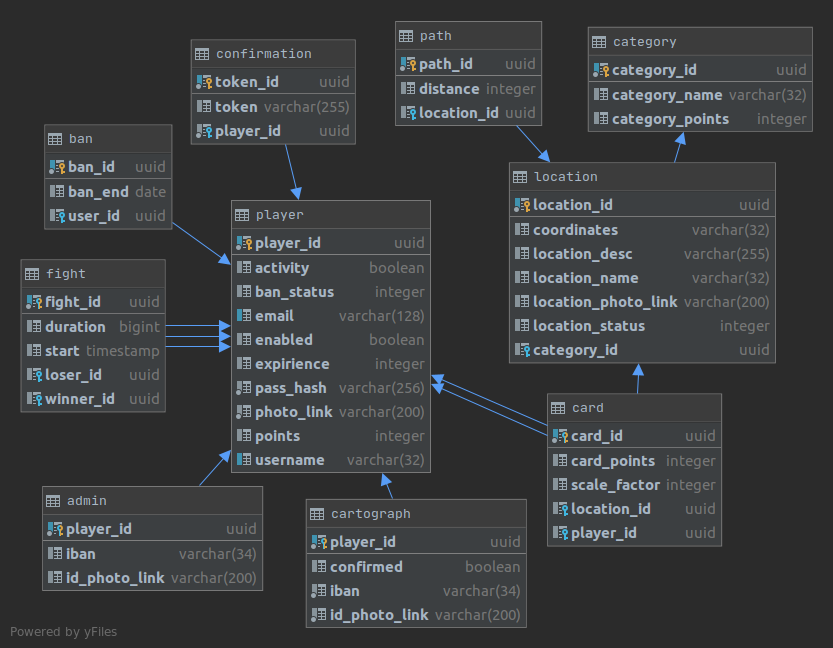
\includegraphics[width=\linewidth, height=14cm]{dijagrami/geofighterdb_diagram}				
					\centering
					\caption{E-R dijagram baze podataka}
					\label{}
				\end{figure}
			
			\eject
			
			
		\section{Dijagram razreda}
		
			{Slike 4.2, 4.3, 4.4 i 4.5 prikazuju razrede \textit{backend} dijela MVC arhitekture. Razredi na slici 4.2 i 4.3 prikazuju razrede Service i razrede Controller s anotacijom @RestController što je specifično za spring boot koji tom anotacijom kombinira anotacije @Controller i @ResponseBody te omogućuje da svaka metoda koja rukuje sa zahtjevima automatski serijalizira povratne vrijednosti objekata u \textit{HttpResponse}. Service razredi služe za modeliranje logike koja se događa nad modelima (npr. slanje mail-a) i služe za odvajanje takve logike od kontrolera čija je zadaća isključivo odgovarati na http zahtjeve (bilo GET, POST, PUT, PATCH ili DELETE).}
			
			\begin{figure}[H]
				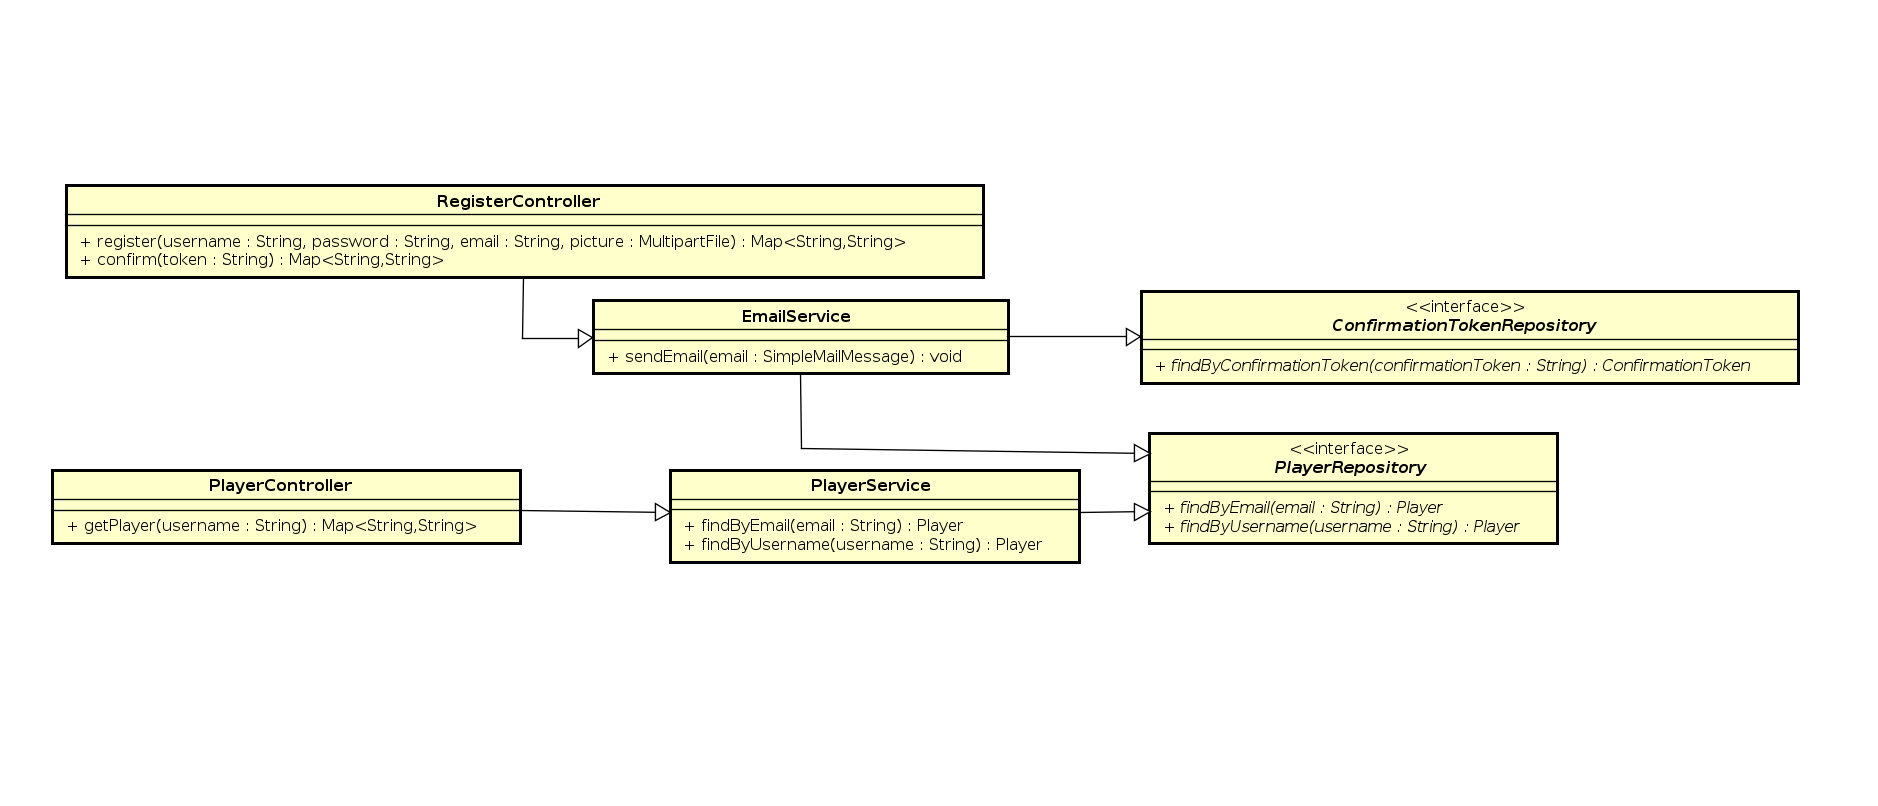
\includegraphics[width=17cm, height=10cm]{dijagrami/servicecontroller_diagram}				
				\centering
				\caption{Dijagram razreda - dio trenutnih Controllers i Service razreda}
				\label{}
			\end{figure}
		
			\begin{figure}[H]
				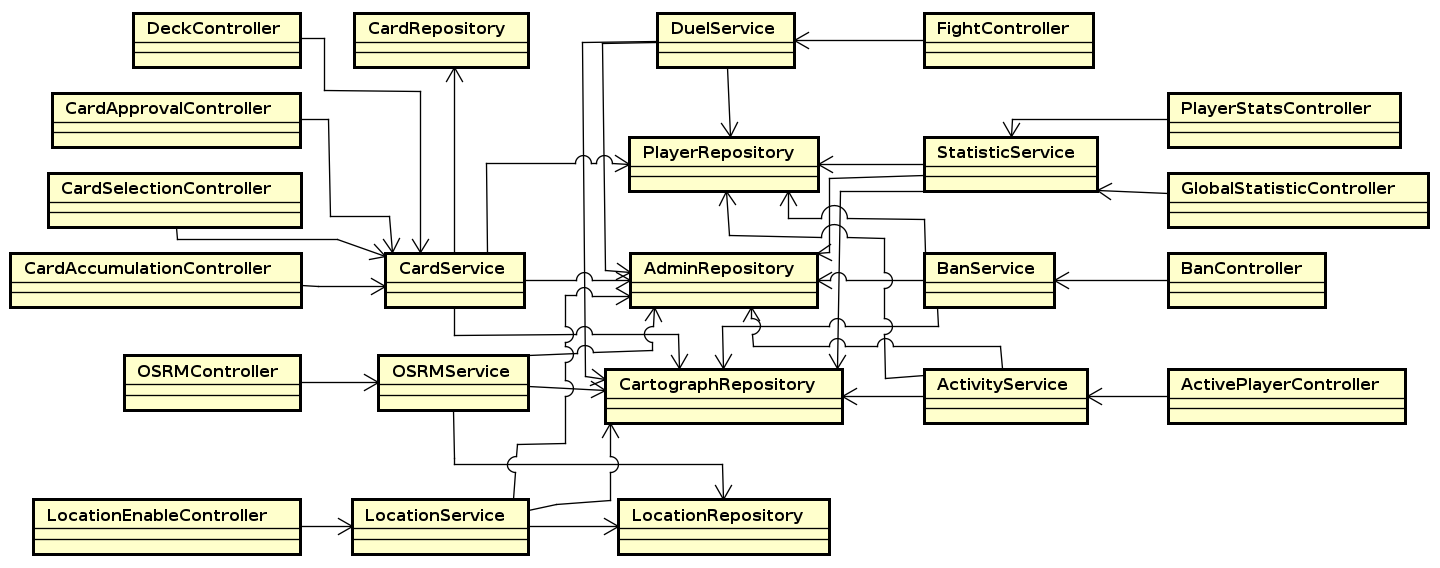
\includegraphics[width=\linewidth, height=14cm]{dijagrami/futureclass_diagram}				
				\centering
				\caption{Dijagram razreda - dio budućih Controller i Service razreda}
				\label{}
			\end{figure}
			
			\begin{figure}[H]
				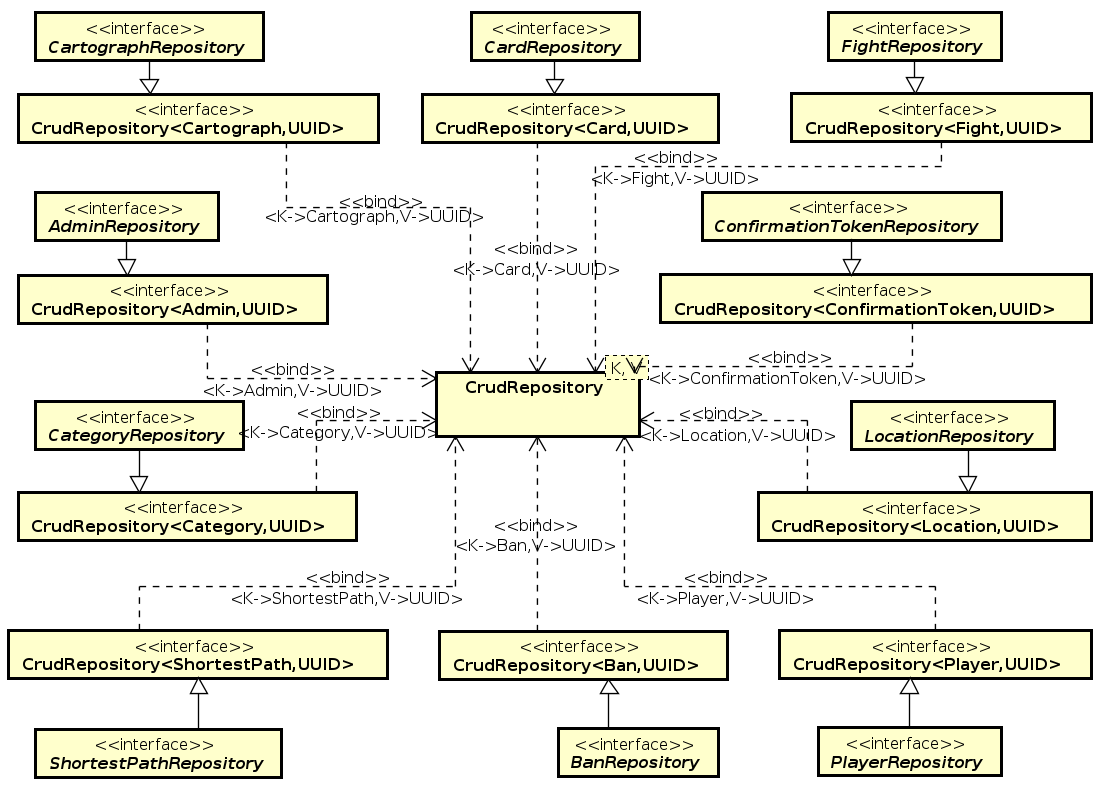
\includegraphics[width=\linewidth, height=14cm]{dijagrami/daoclass_diagram}				
				\centering
				\caption{Dijagram razreda - dio Data access object razreda}
				\label{}
			\end{figure}
		
			{Model razredi preslikavaju strukturu baze podataka aplikacije. Razred Player predstavlja igrača koji se može registrirati, raspolaže svojim špilom karata koje skuplja te sudjeluje u borbama i otkrivanju novih lokacija. Razred Admin predstavlja administratora te nasljeđuje sve funkcije razreda Player i ima sve ovlasti nad bazom podataka i upravljanja igračima svih razina. Razred Cartograph predstavlja kartografa koji nasljeđuje sve funkcije razreda Player i ima mogućnosti upravljanja svim postojećim i novim lokacijama. Razred Fight predstavlja borbu u kojoj sudjeluju dva igrača. Razred Card predstavlja kartu koja obzirom na kategoriju lokacije kojoj pripada sadrži određen broj bodova koji se koristi u borbama. Razred Location predstavlja lokaciju na kojoj se mogu skupljati karte ukoliko ih kartograf odobri. Razred Category predstavlja kategoriju lokacije prema čijoj se klasifikaciji određuje broj bodova koje lokacije donose.}
			
			\begin{figure}[H]
				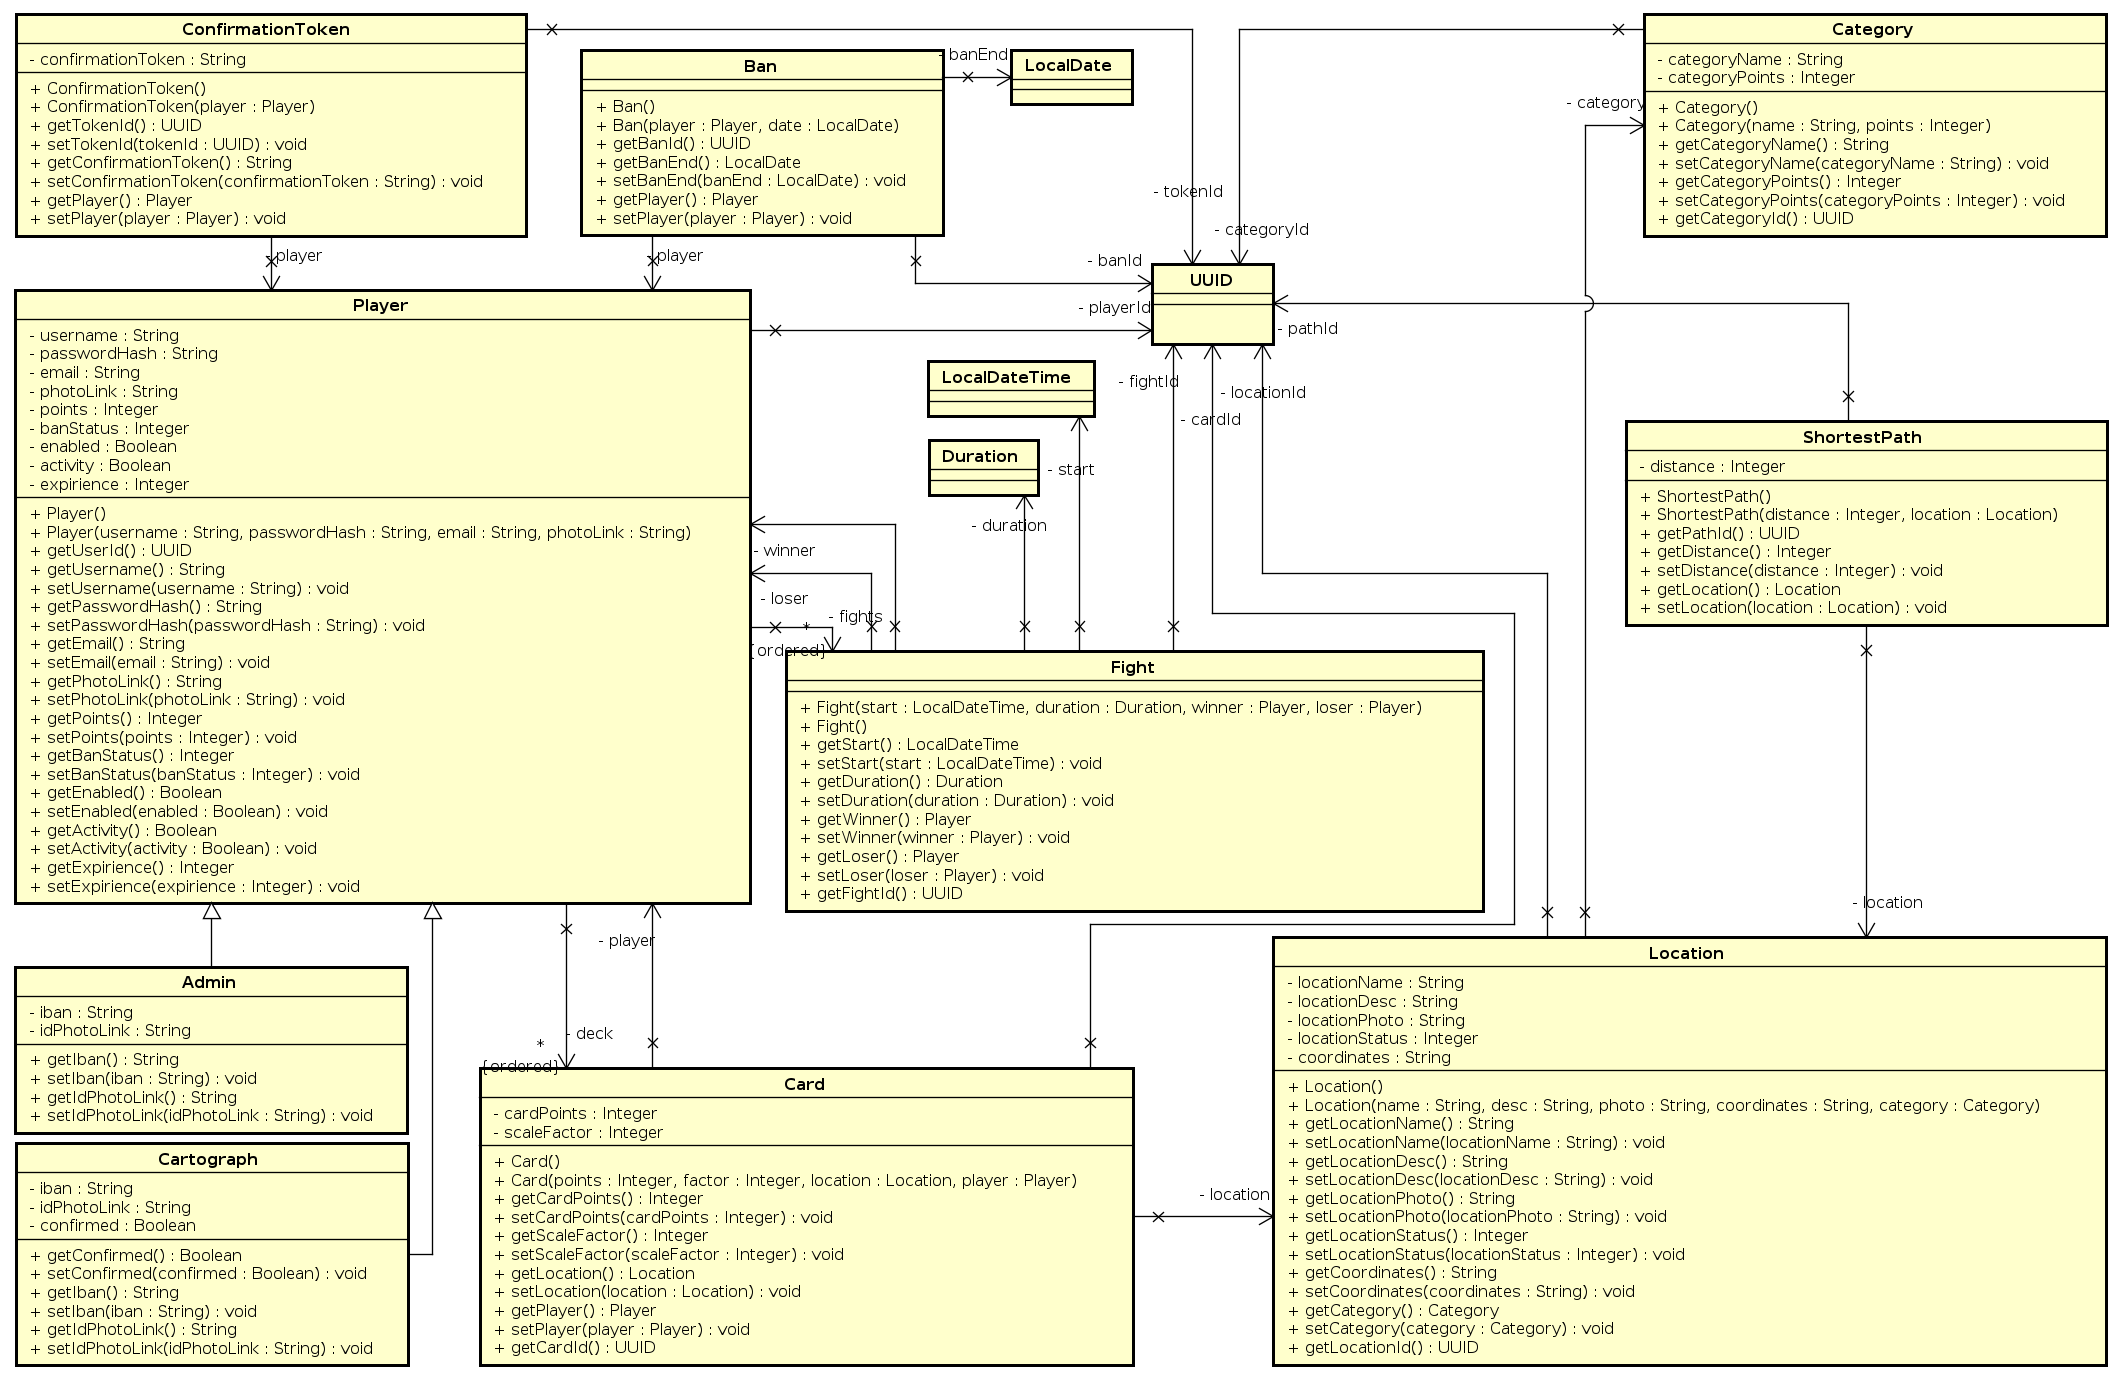
\includegraphics[width=\linewidth, height=14cm]{dijagrami/modelclass_diagram}				
				\centering
				\caption{Dijagram razreda - dio Models razreda}
				\label{}
			\end{figure}
			
			\textbf{\textit{dio 2. revizije}}\\			
			
			\textit{Prilikom druge predaje projekta dijagram razreda i opisi moraju odgovarati stvarnom stanju implementacije}
			
			
			
			\eject
		
		\section{Dijagram stanja}
			
			
			\textbf{\textit{dio 2. revizije}}\\
			
			\textit{Potrebno je priložiti dijagram stanja i opisati ga. Dovoljan je jedan dijagram stanja koji prikazuje \textbf{značajan dio funkcionalnosti} sustava. Na primjer, stanja korisničkog sučelja i tijek korištenja neke ključne funkcionalnosti jesu značajan dio sustava, a registracija i prijava nisu. }
			
			
			\eject 
		
		\section{Dijagram aktivnosti}
			
			\textbf{\textit{dio 2. revizije}}\\
			
			 \textit{Potrebno je priložiti dijagram aktivnosti s pripadajućim opisom. Dijagram aktivnosti treba prikazivati značajan dio sustava.}
			
			\eject
		\section{Dijagram komponenti}
		
			\textbf{\textit{dio 2. revizije}}\\
		
			 \textit{Potrebno je priložiti dijagram komponenti s pripadajućim opisom. Dijagram komponenti treba prikazivati strukturu cijele aplikacije.}